\documentclass[12pt]{article}
\usepackage{graphicx}
\usepackage{subcaption}
\usepackage{float}
\usepackage{hyperref}

\title{EE236: Experiment 10\\
C-V characteristics of MOSCAP}

\author{Aaron John Sabu, 170070050}

\begin{document}
\maketitle

\section{Aim of the experiment}

The experiment aims to realise the C-V Characteristics of a MOSCAP (Metal Oxide Semiconductor CAPacitor).\\
Based on the same, the experiment also aims on calculating different parameters of the MOSCAP such as oxide capacitance, oxide thickness, flat-band voltage, flat-band capacitance, doping density and built-in voltage.

\section{Methods}
The experiment was performed using TL071 opamp ICs, resistances of various values and capacitors. A circular metalized region from the MOSCAP sample surface was chosen and the POGO contact needle was place well within the boundaries of this region.\\
The voltmeters were used via the portable Digital Multimeter and the provided multimeter. The circuit was connected as shown below:
\begin{figure}[H]
	\centering
	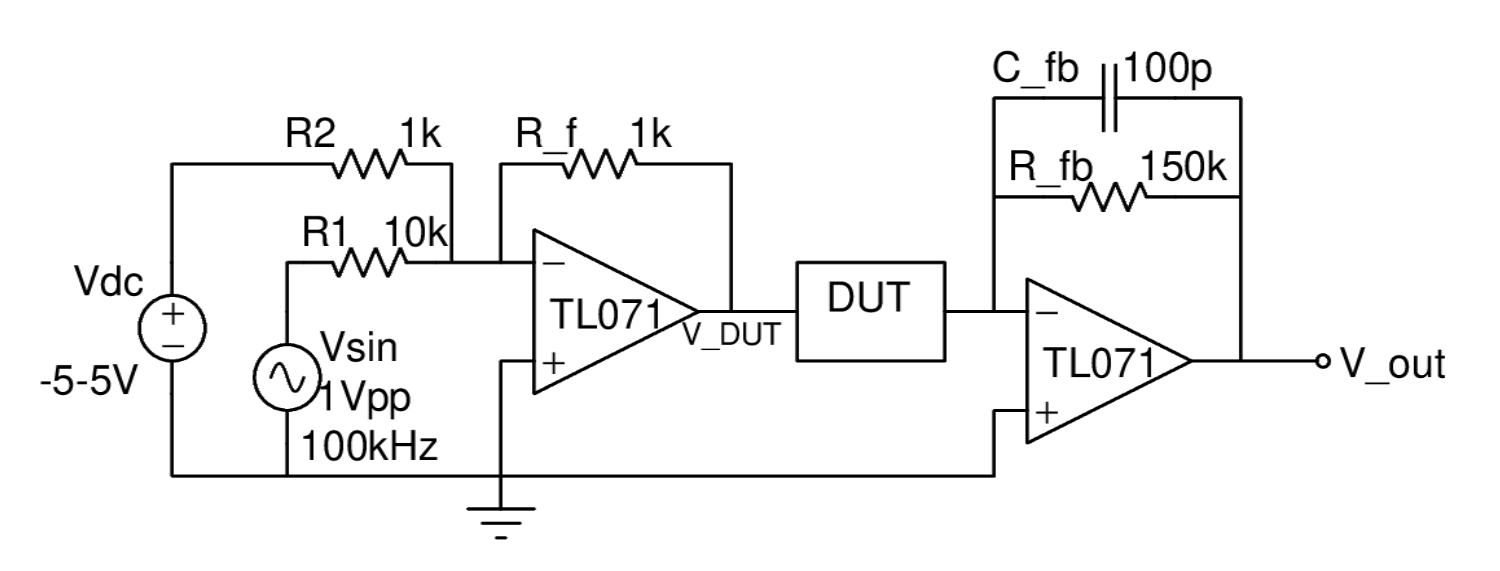
\includegraphics[width = \linewidth, trim = {0 0 0 0}, clip]{Circuit_Diagram.png}
	\caption{Circuit Diagram}
\end{figure}

The experiment was performed in room temperature and normal laboratory conditions.\\
The AC voltage is scaled down 10 times and the DC voltage is kept as it is. The two are summed up as the output of the summer. The current flowing through the device under test is amplified and is measured as voltage at \(V_{out}\).

\section{Observations}

\subsection{Summer Circuit}

From the given plots we realise that the summer circuit added the DC voltage and the scaled down AC voltage properly:
\begin{figure}[H]
	\centering
	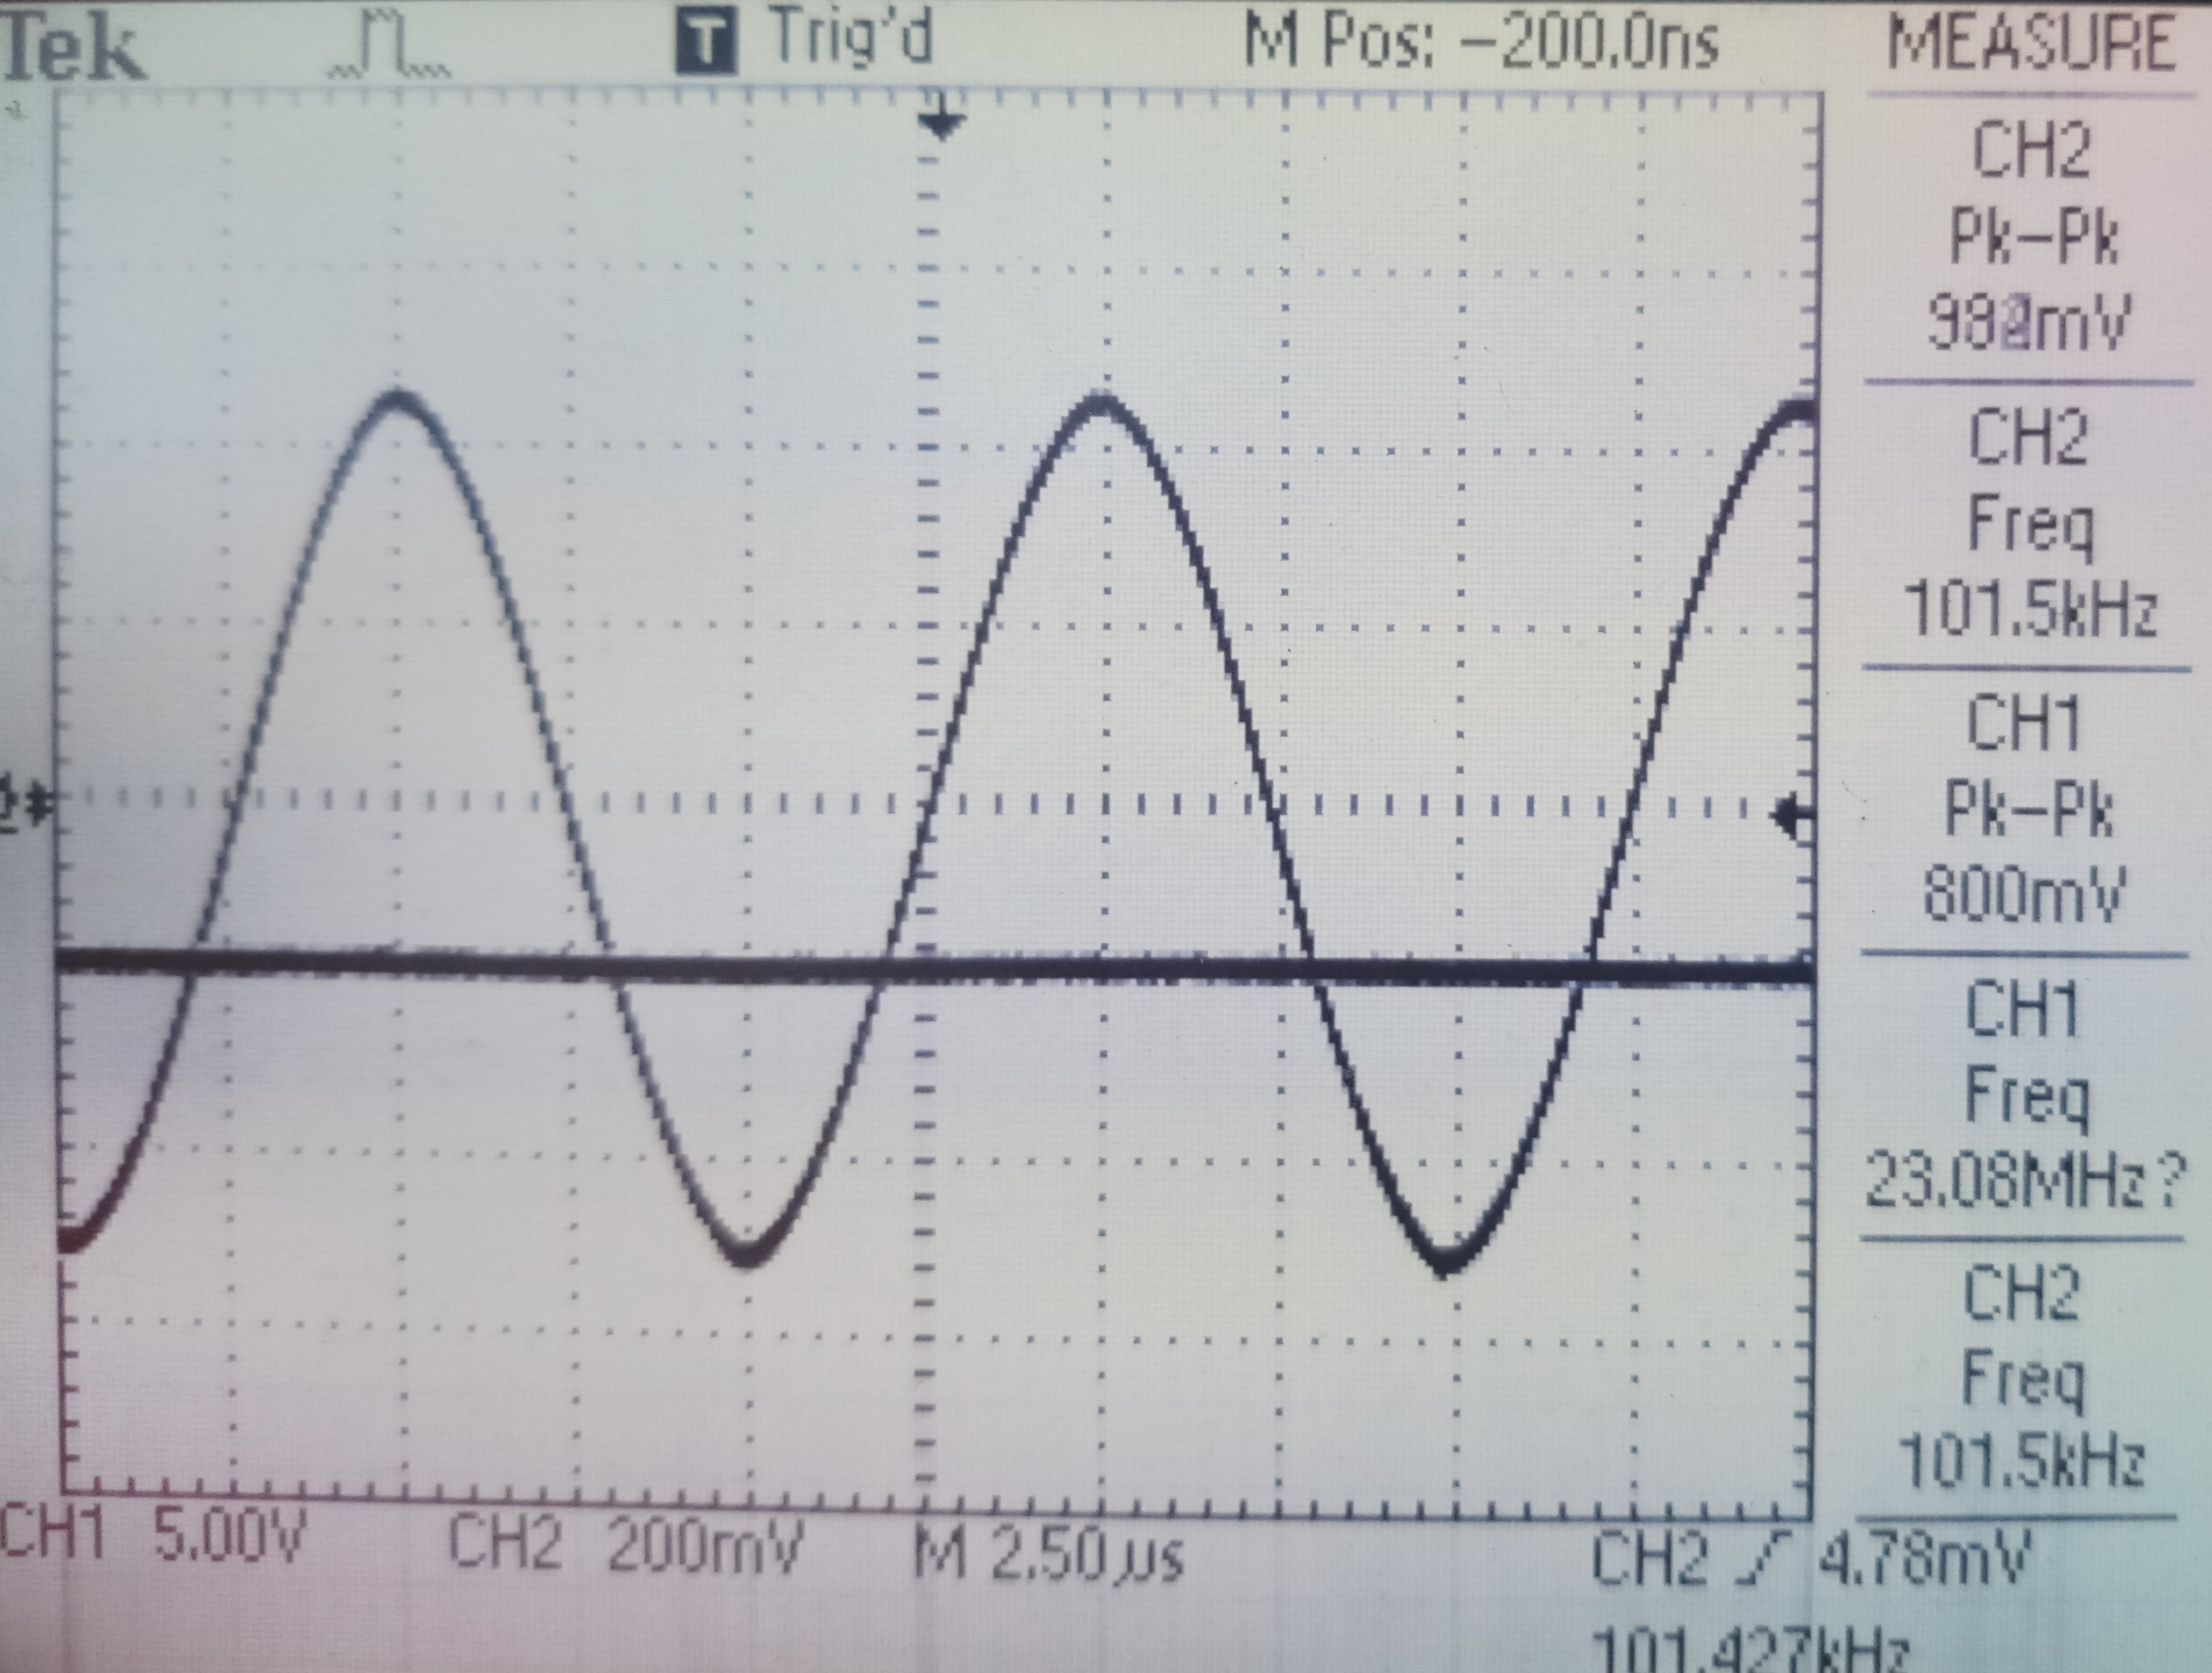
\includegraphics[width = 0.8\linewidth, trim = {0 0 0 0}, clip]{14_45_57.jpg}
	\caption{DC Output}
\end{figure}
\begin{figure}[H]
	\centering
	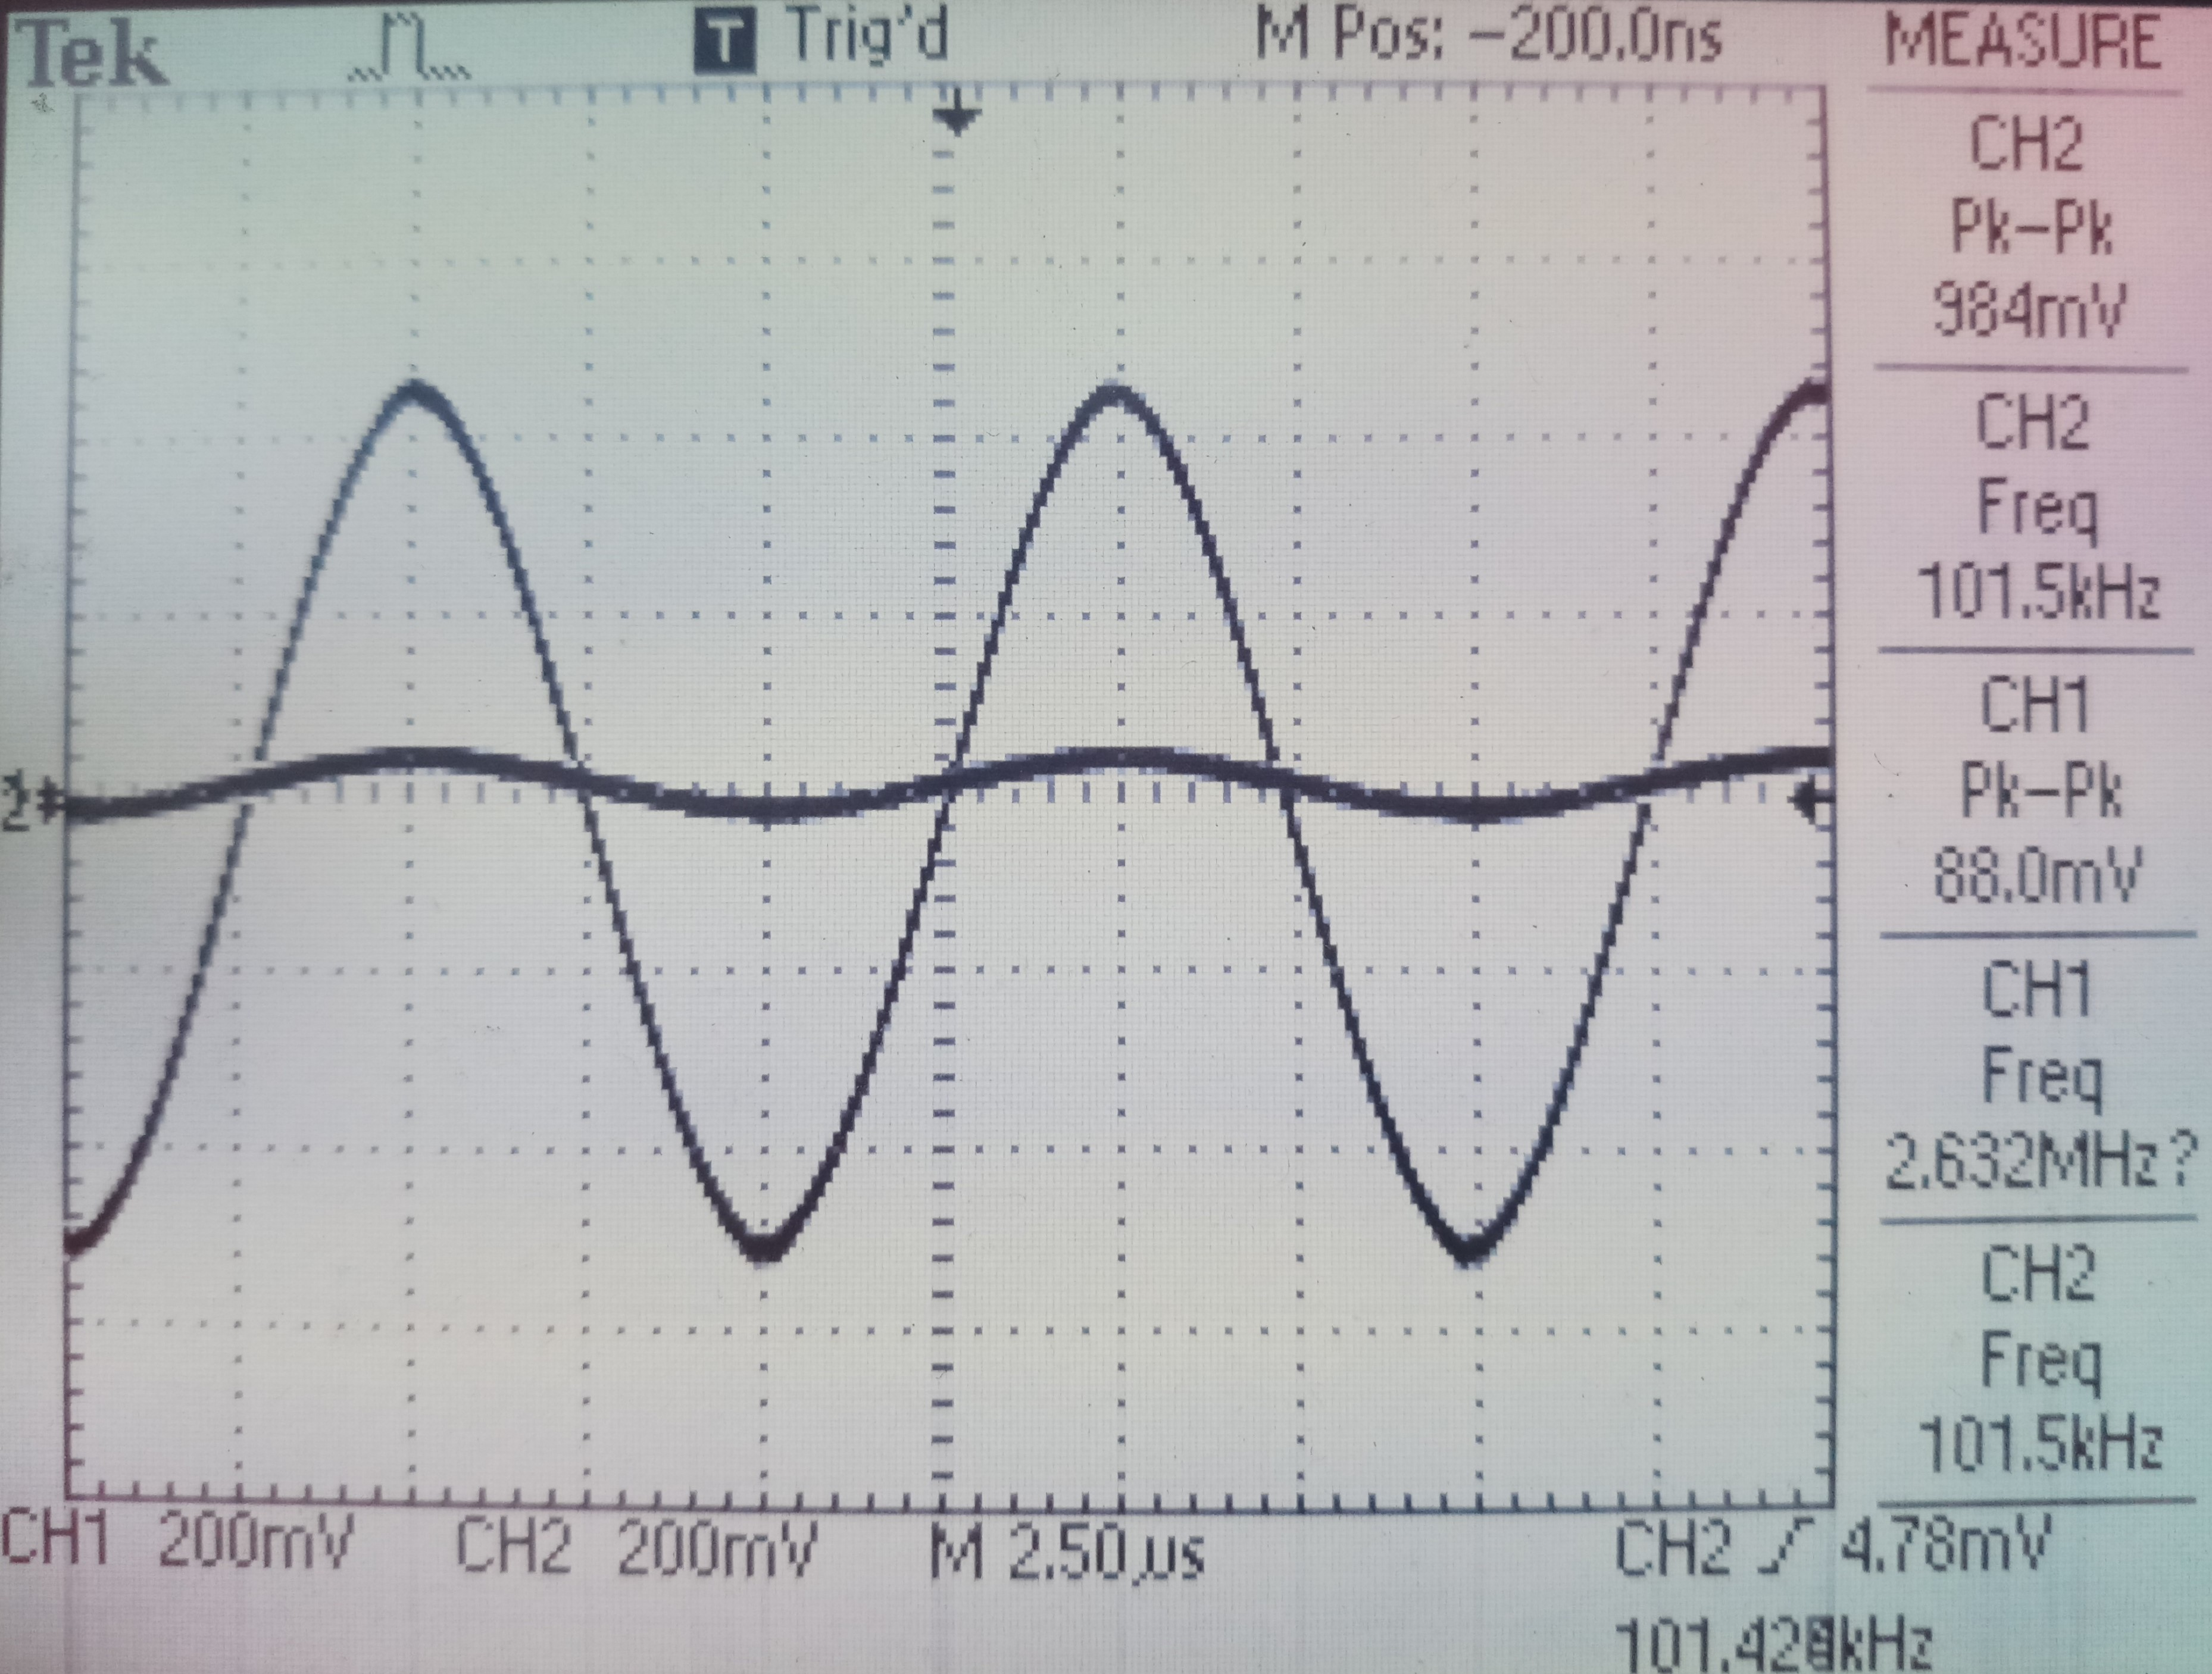
\includegraphics[width = 0.8\linewidth, trim = {0 0 0 0}, clip]{14_46_48.jpg}
	\caption{AC Output}
\end{figure}

\subsection{Amplifier Circuit}

From the given plots we realise that the summer circuit functioned properly, hence providing the correct value of the test capacitance. The two DSO figures below  were taken for \(C_{DUT}\) = 100 pF
\begin{center}
\begin{figure}[H]
	\begin{subfigure}[b]{\linewidth}
	   	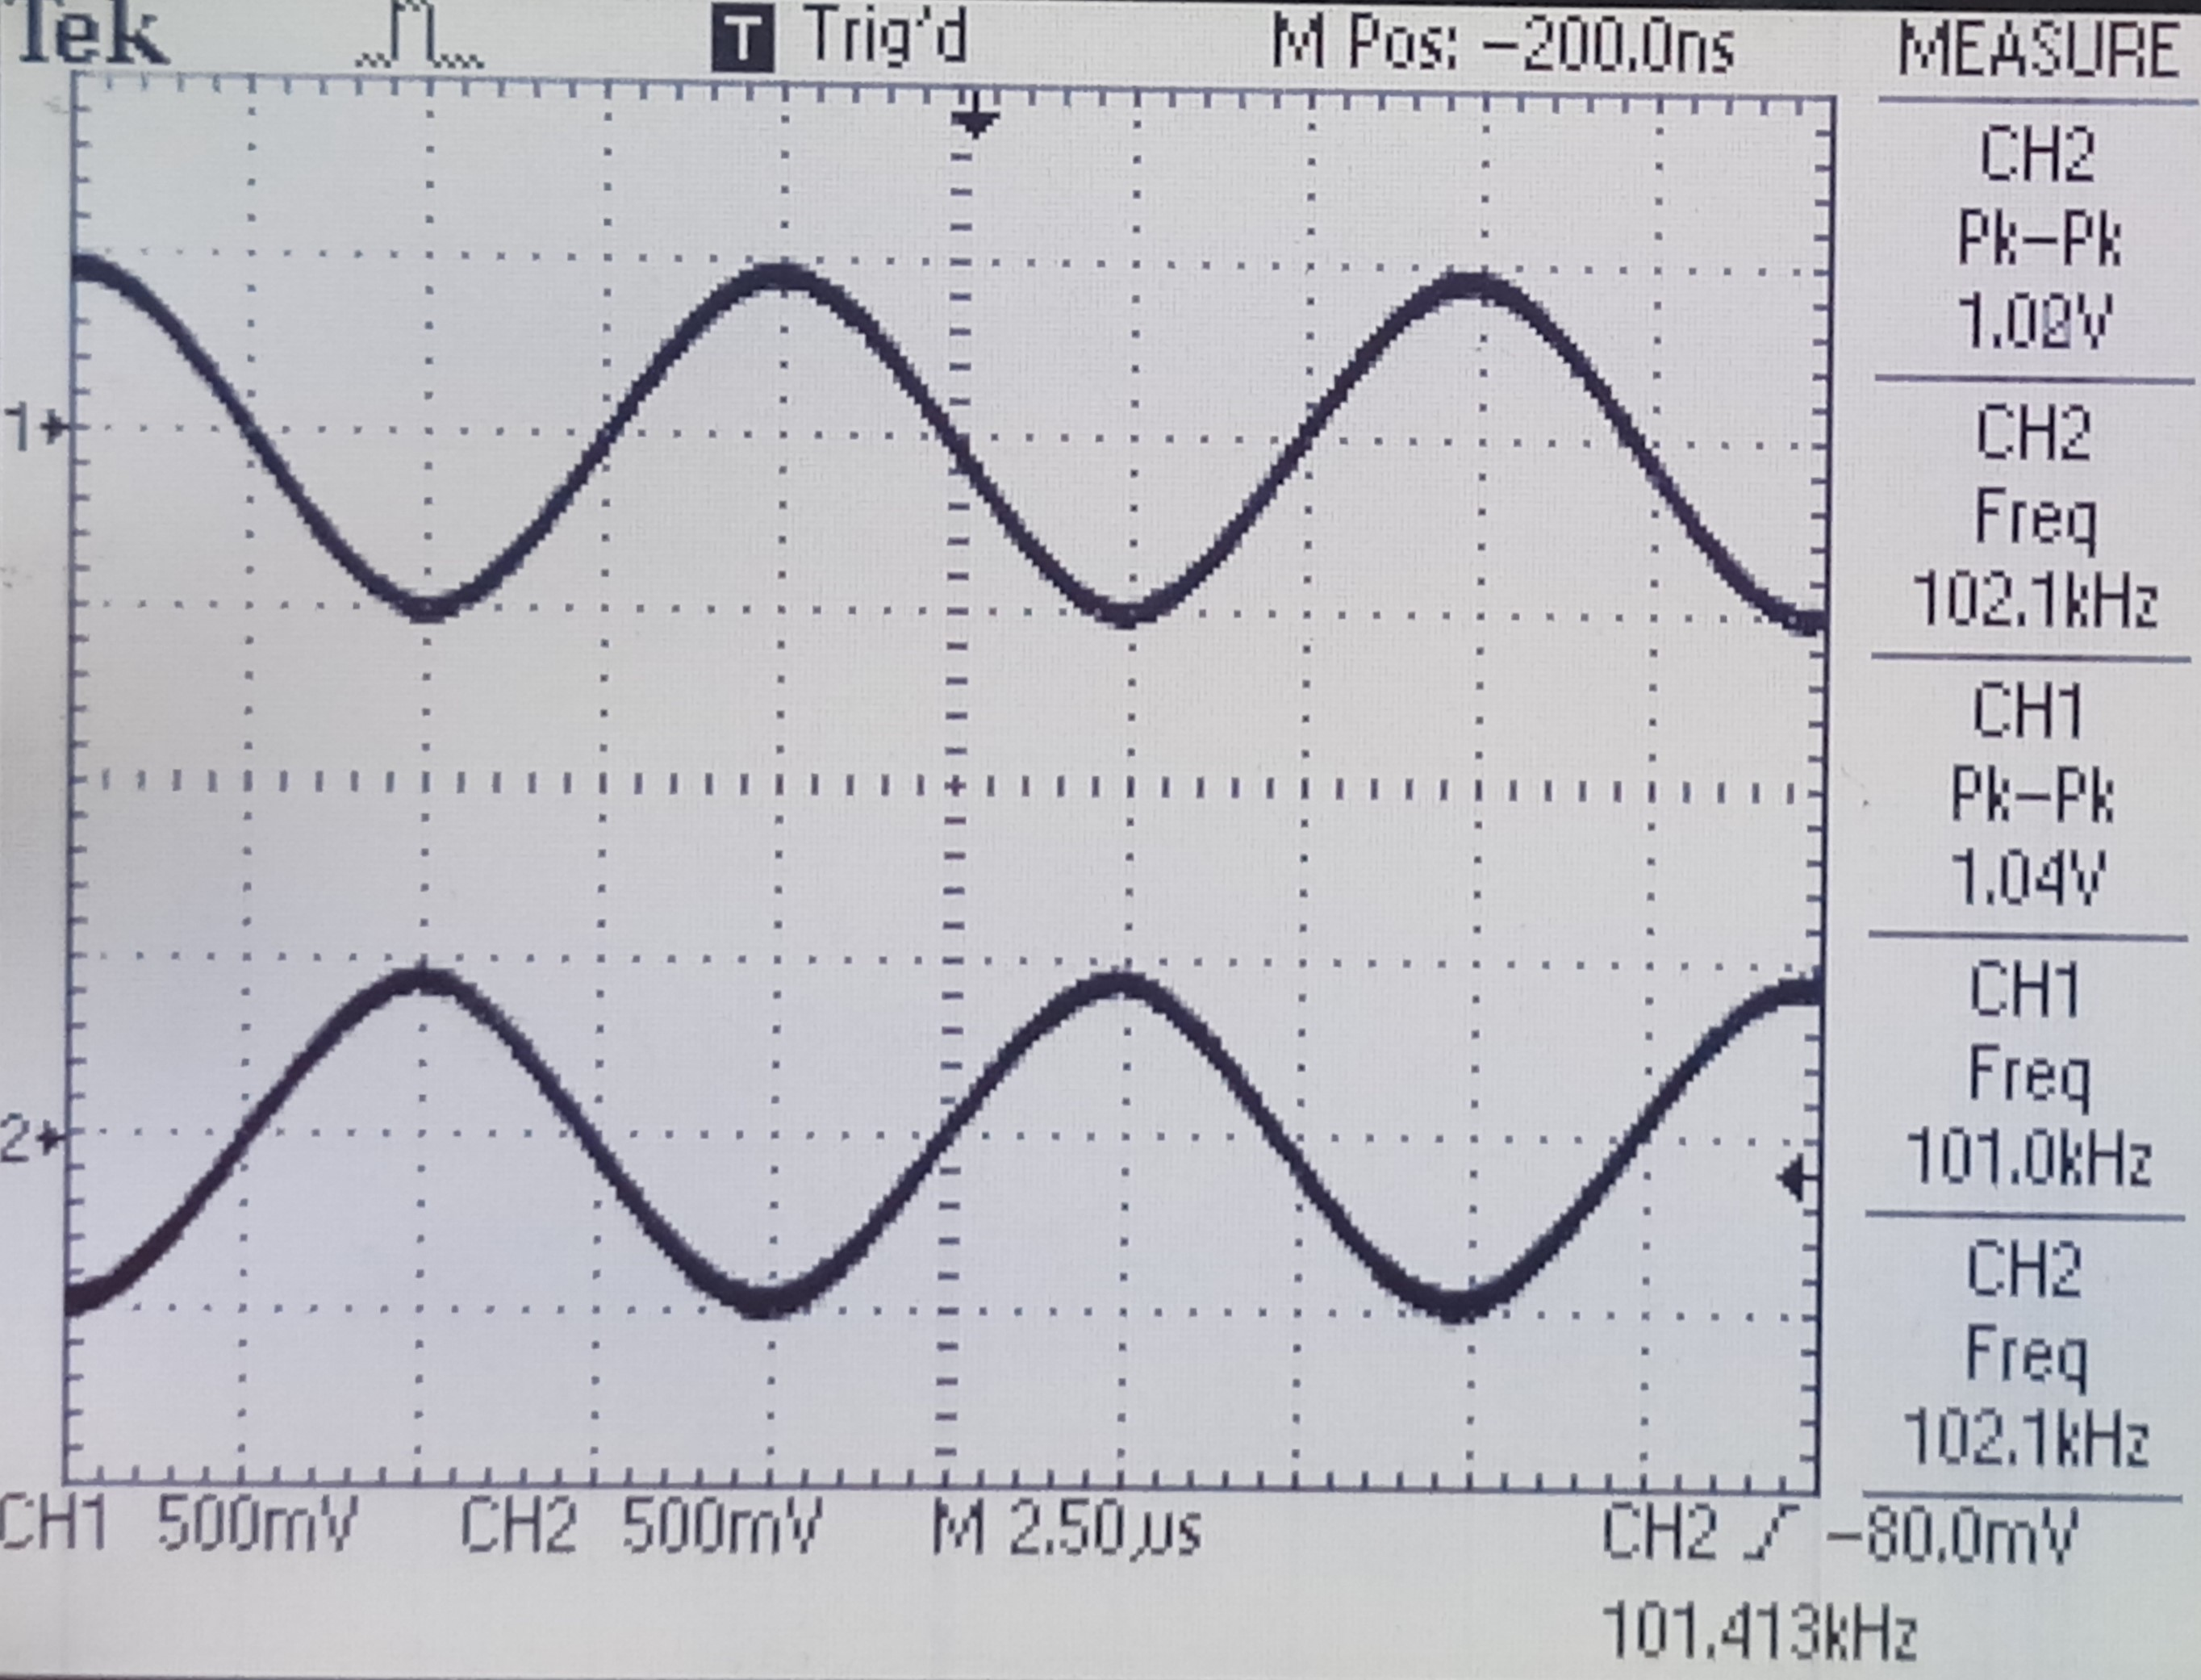
\includegraphics[width = 0.65\linewidth, trim = {0 0 0 0}, clip]{14_56_42.jpg}
		\caption{\(C_{fb}\) = 100 pF}
	\end{subfigure}\\
	\begin{subfigure}[b]{\linewidth}
	   	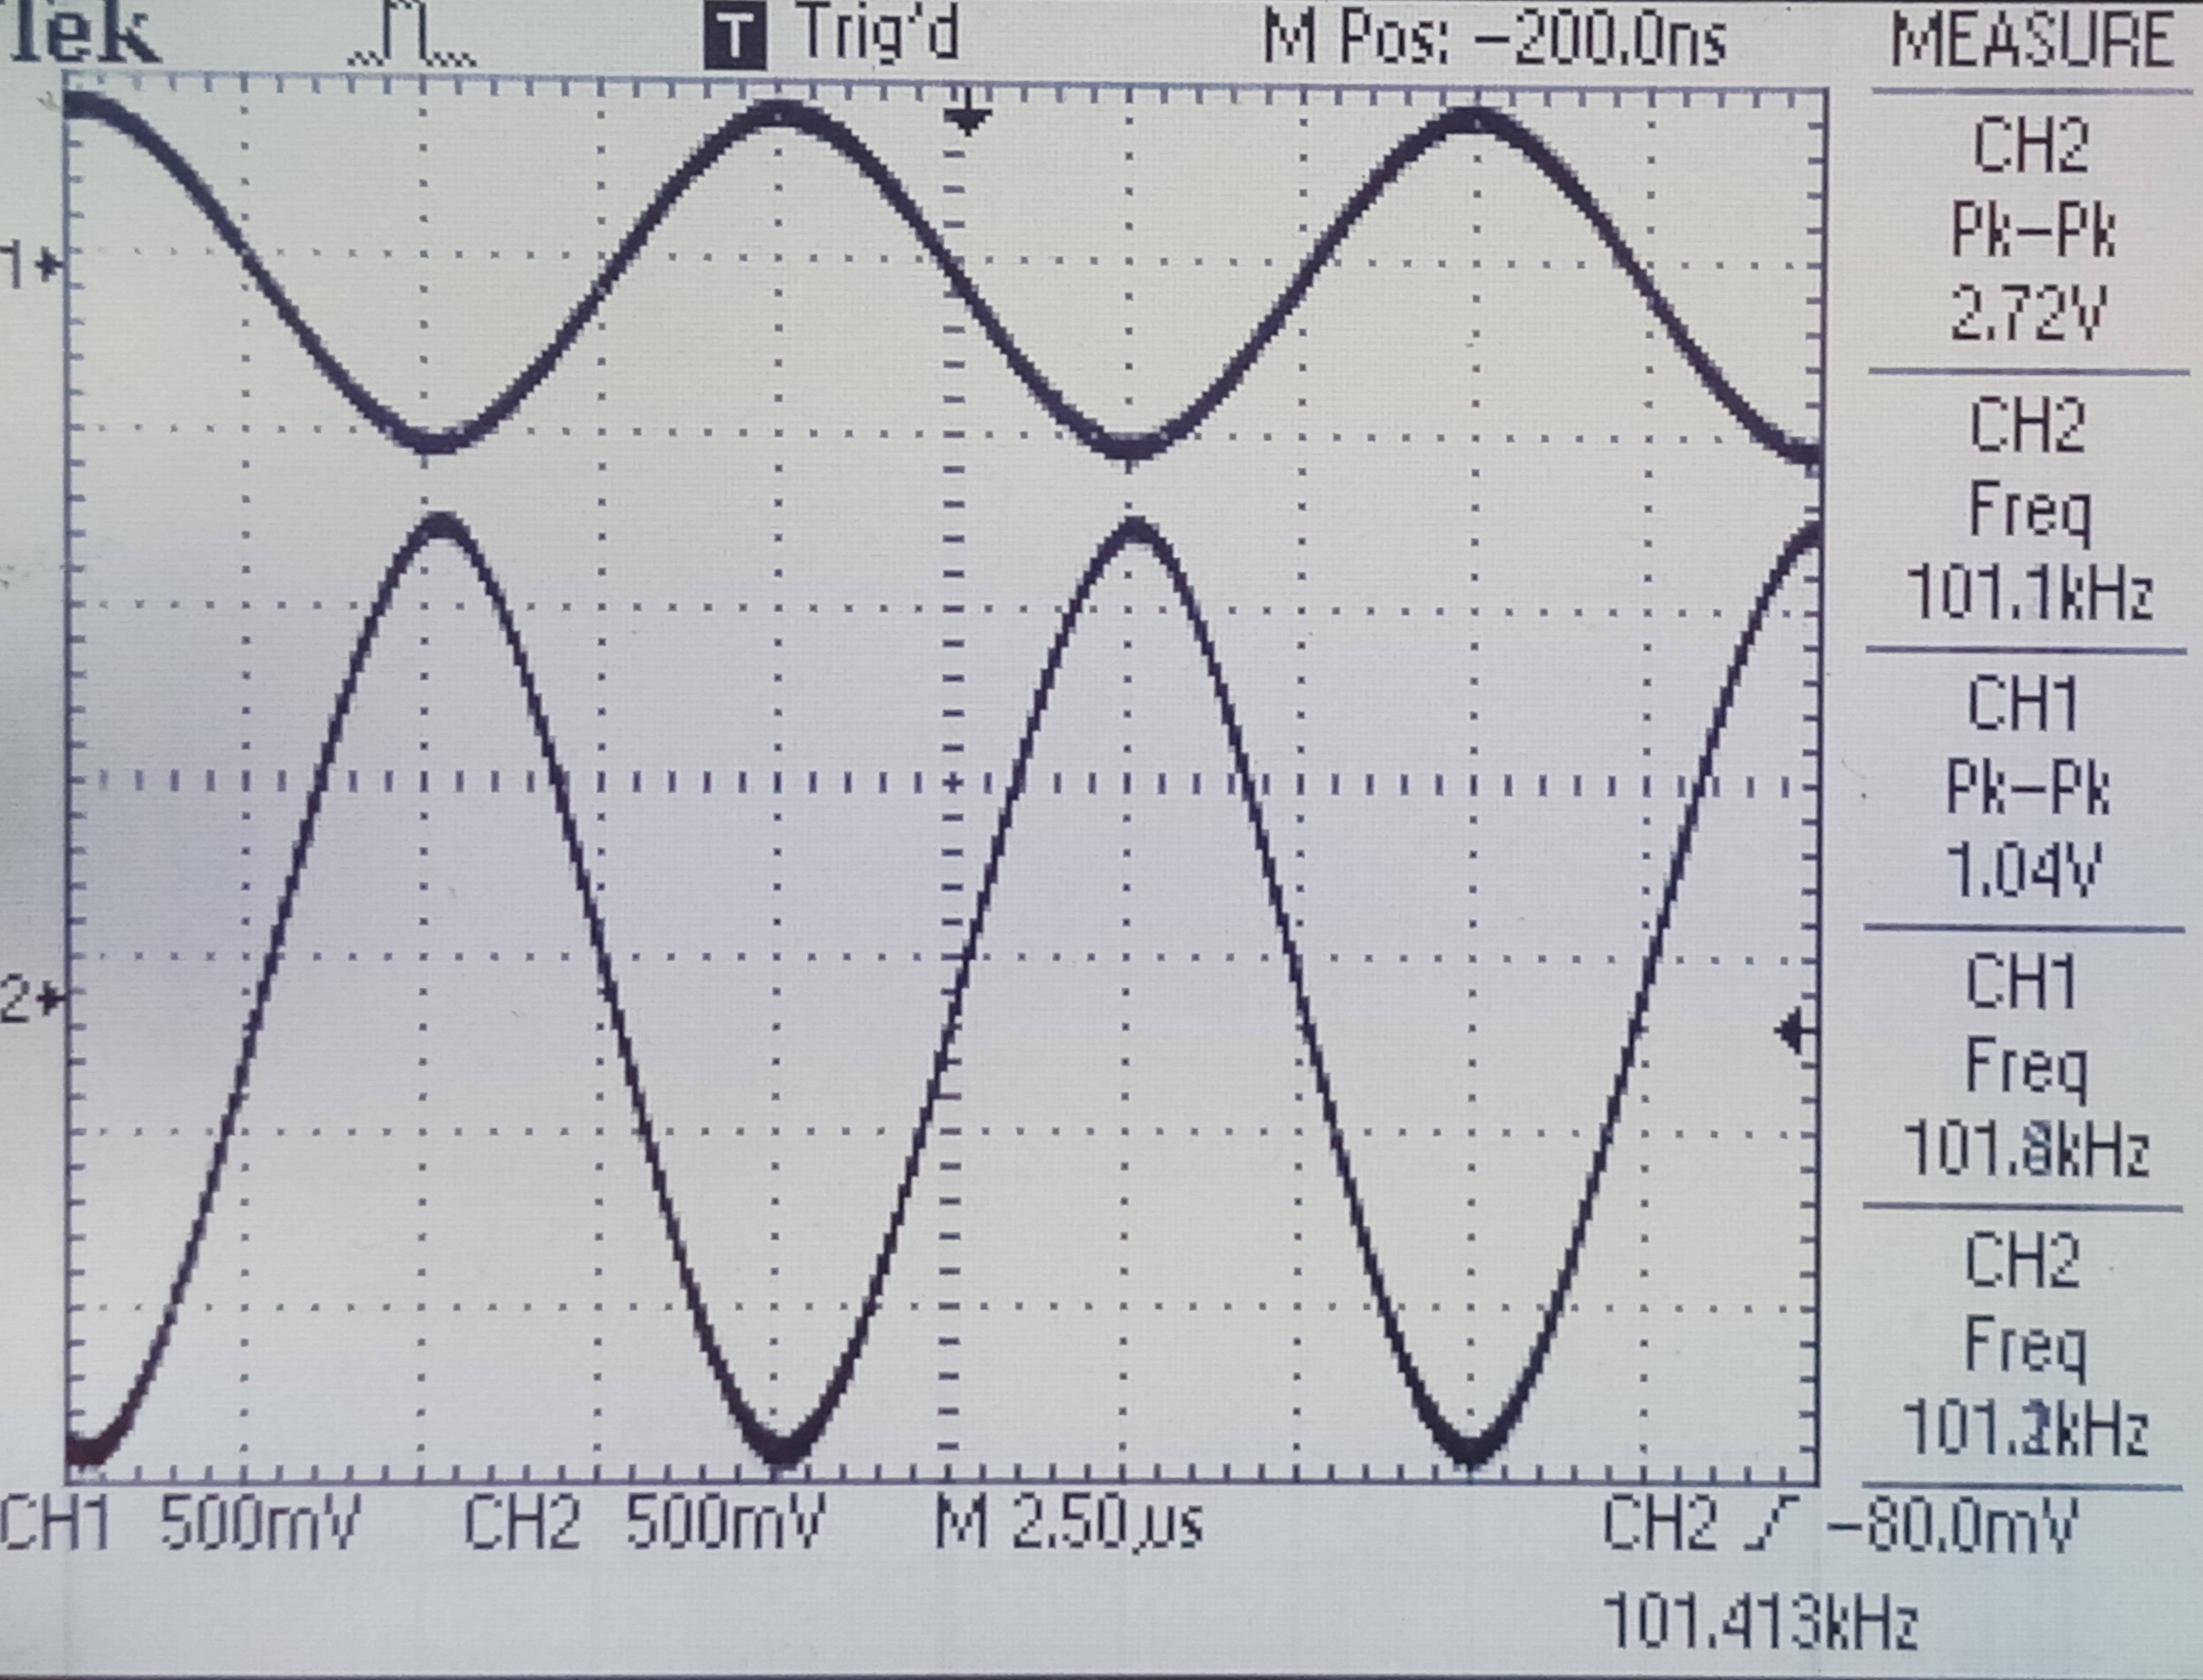
\includegraphics[width = 0.65\linewidth, trim = {0 0 0 0}, clip]{14_57_31.jpg}
		\caption{\(C_{fb}\) = 330 pF}
	\end{subfigure}\\
	\caption{DSO Output for \(C_{DUT}\) = 100 pF}
\end{figure}
\end{center}

\subsection{Device Under Test (DUT) Circuit}

The frequency used was 100 kHz. Hence we get \(\omega = 6.28 \times 10^5 s^{-1}\). The values of \(V_{out}\) are not mentioned for \(V_{DC} > 0 V\) because they were not measured in the laboratory. Rather than using the values provided for the batch due to mismatch of values, the capacitance values in the positive region were assumed to be constant due to large variations from the values provided from the previous batch. Using these values, we can calculate the values of capacitance for each value of \( V_{DC} \):
\[C_{DUT} = C_{fb} \times \frac{V_{out}} {V_{DUT}} \times \left(1+\left(\frac{1}{\omega*R_{fb}*C_{fb}}\right)^2\right)^{0.5}\]

\begin{center}
 \begin{tabular}{|| c | c | c || c | c | c ||} 
 \hline
 \hline
 \( V_{DC} (V) \) & \( V_{out} (V) \) & \( C (pF) \) & \( V_{DC} (V) \) & \( V_{out} (V) \) & \( C (pF) \) \\ [0.25ex] 
 \hline\hline
 \hline 
5 & - & 230.77 & -1 & 208 & 209.17 \\ \hline
4.5 & - & 230.77 & -1.3 & 196 & 197.1 \\ \hline
4 & - & 230.77  & -1.5 & 208 & 209.17  \\ \hline
3.5 & - & 230.77  & -1.6 & 226 & 227.27  \\ \hline
3 & - & 230.77 & -1.7 & 234 & 235.31 \\ \hline
2.5 & - & 230.77 & -1.8 & 250 & 251.4 \\ \hline
2 & - & 230.77 & -1.9 & 264 & 265.48 \\ \hline
1.5 & - & 230.77 & -2 & 298 & 299.67  \\ \hline
1 & - & 230.77  & -2.1 & 310 & 311.74 \\ \hline
0.5 & - & 230.77 & -2.2 & 316 & 317.77 \\ \hline
0 & - & 230.77 & -2.4 & 336 & 337.89 \\ \hline
-0.1 & 228 & 229.28 & -2.6 & 352 & 353.98 \\ \hline
-0.4 & 220 & 221.23 & -2.8 & 348 & 349.95 \\ \hline
-0.6 & 216 & 217.21 & -3 & 354 & 355.99 \\ \hline
-0.7 & 212 & 213.19 & -3.2 & 358 & 360.01 \\ \hline
- & - & - & -3.4 & 354 & 355.99\\ \hline
\end{tabular}
\end{center}

\begin{figure}[H]
	\centering
	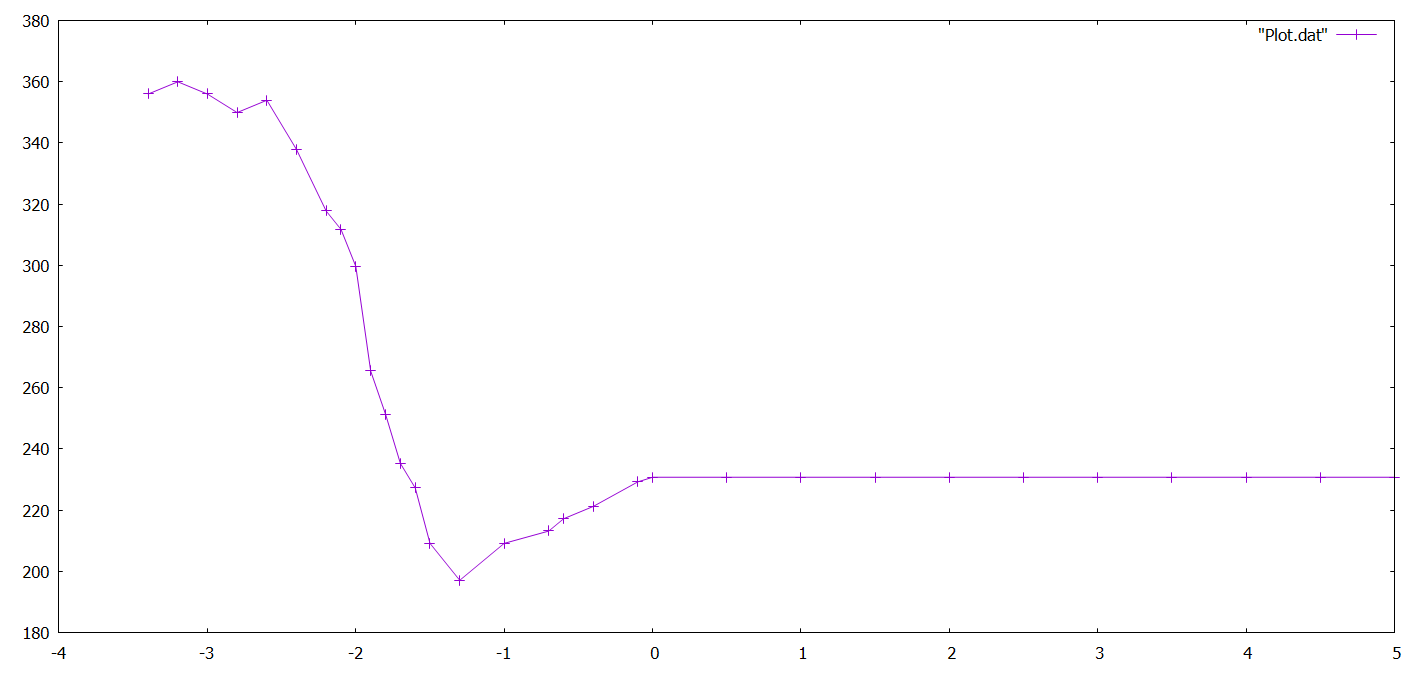
\includegraphics[width = \linewidth, trim = {0 0 0 0}, clip]{Plot.PNG}
	\caption{\(C\) vs \(V_{DC}\)}
\end{figure}

Given below are a few outputs received on the DSO:

\begin{center}
\begin{figure}[H]
	\begin{subfigure}[b]{\linewidth}
	   	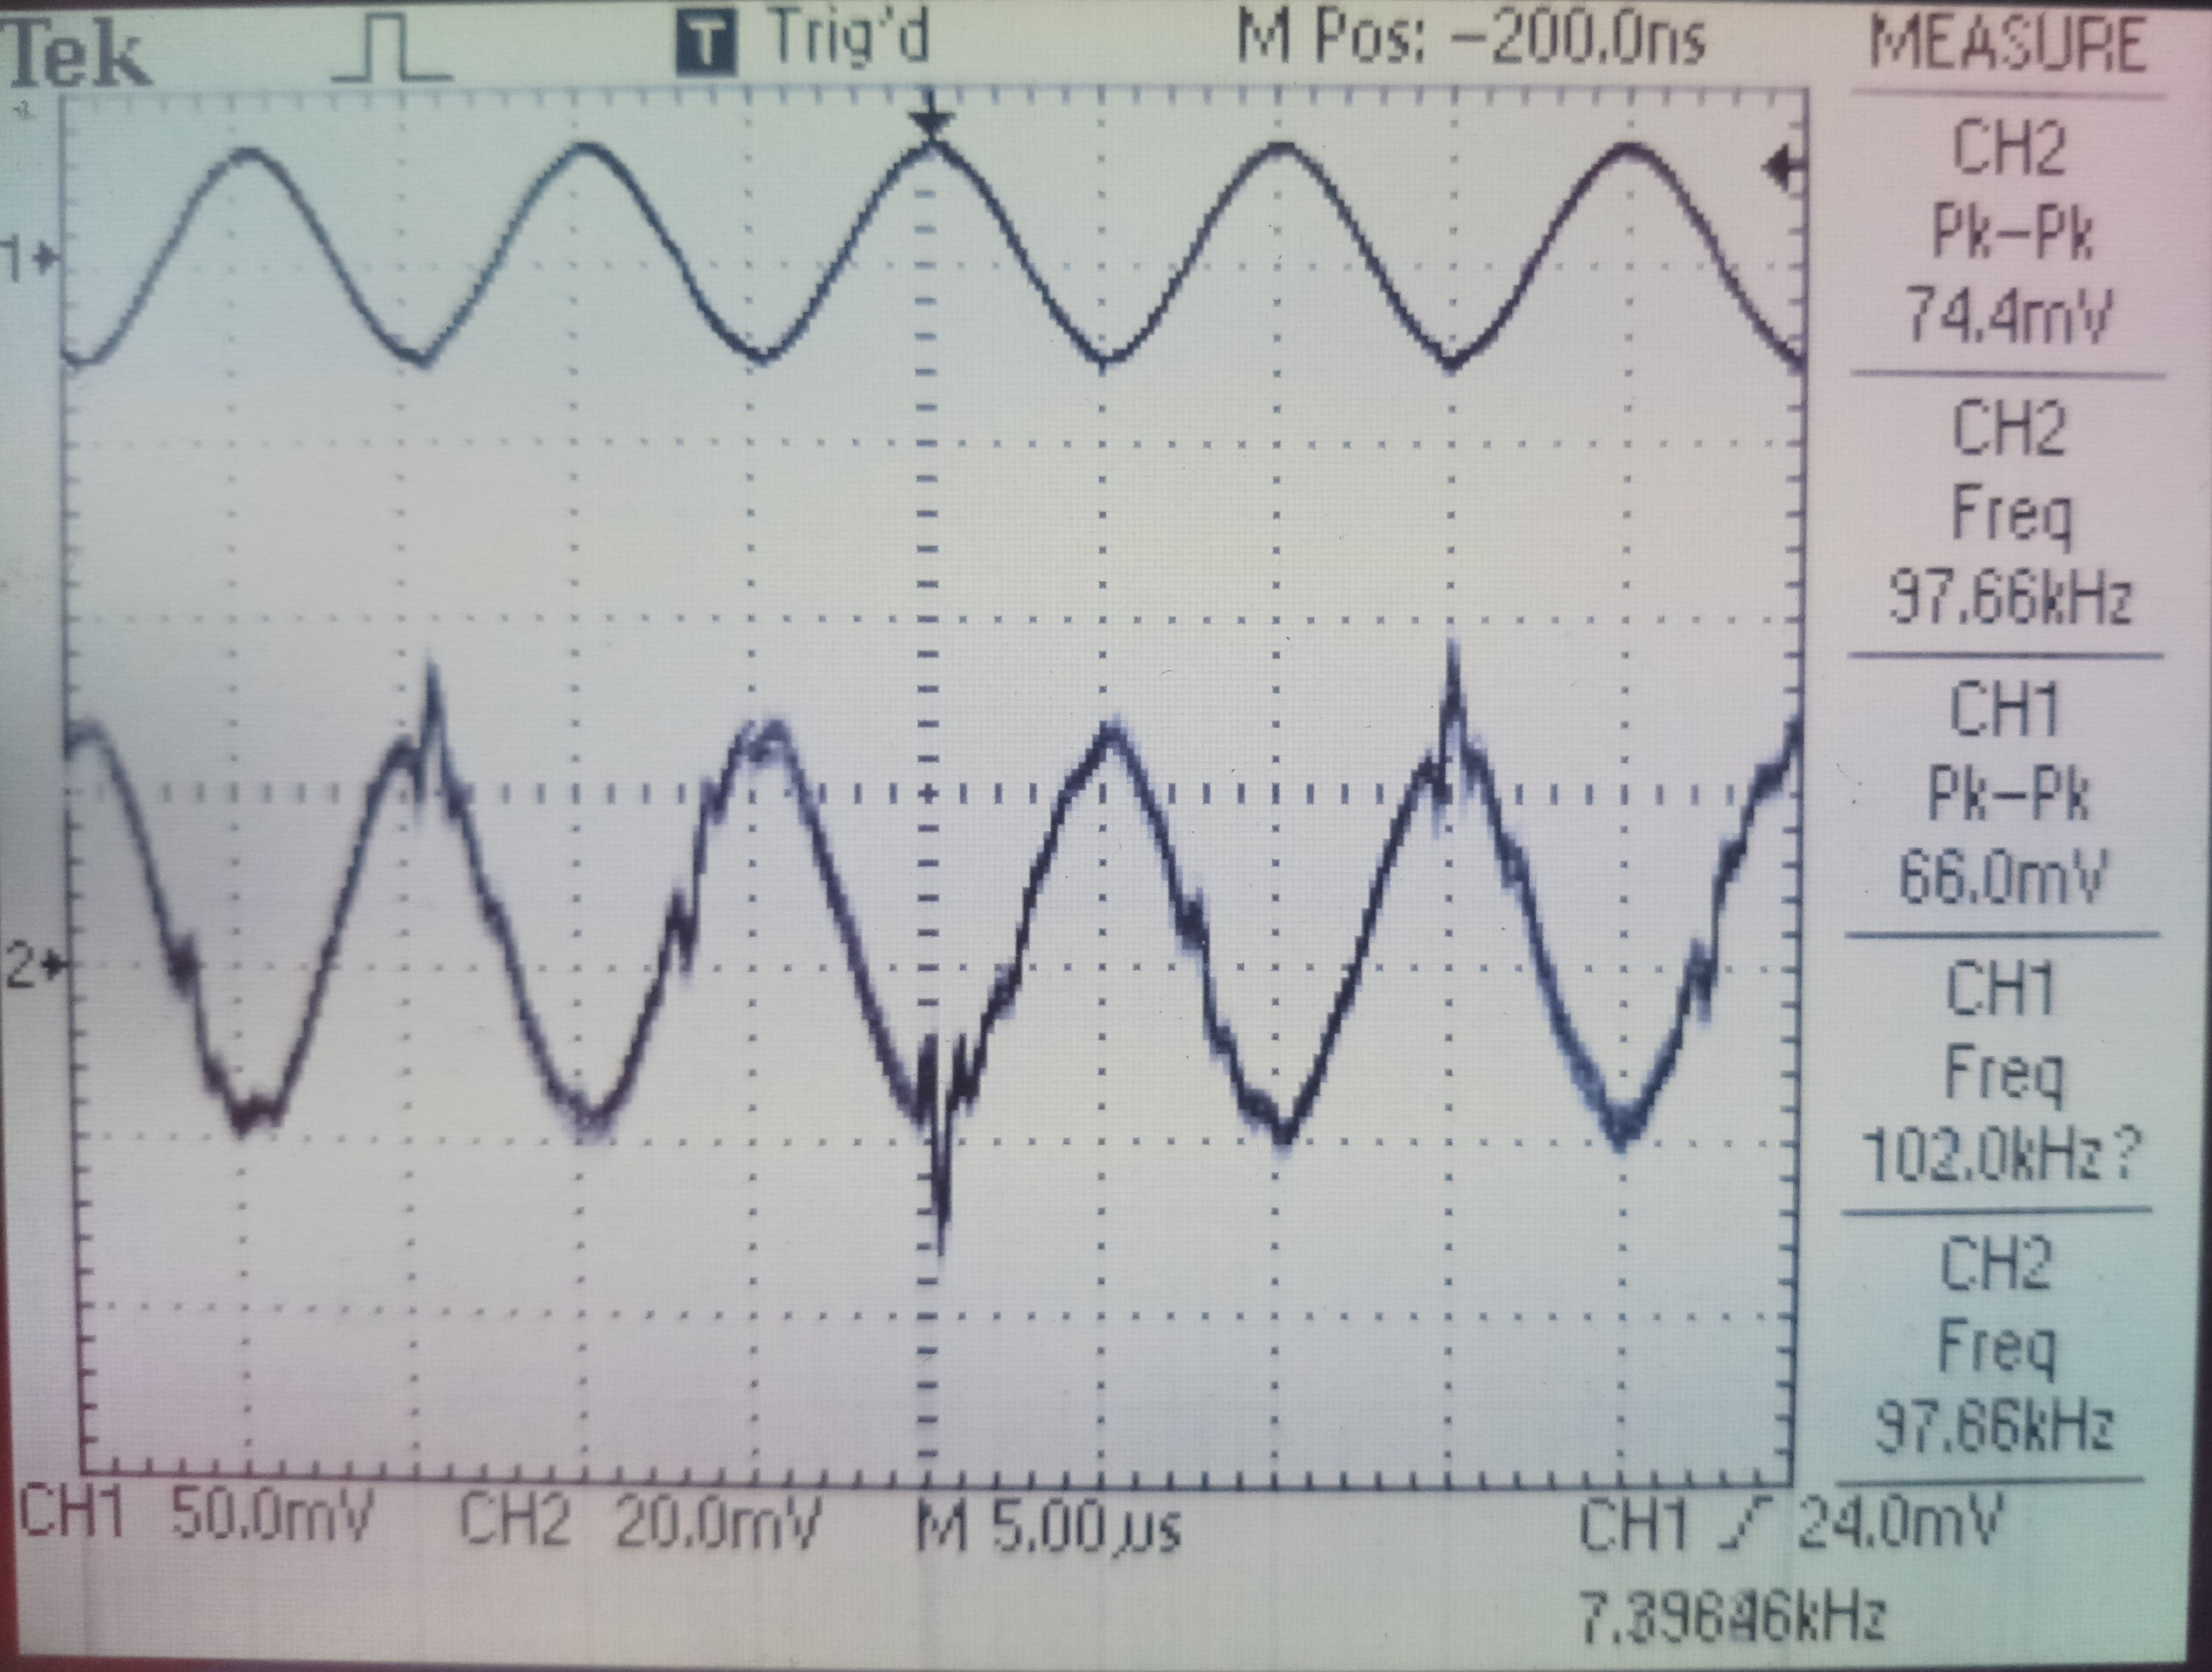
\includegraphics[width = 0.75\linewidth, trim = {0 0 0 0}, clip]{15_22_19.jpg}
		\caption{Observation 1}
	\end{subfigure}\\
	\caption{DUT Outputs}
\end{figure}
\begin{figure}[H]
	\begin{subfigure}[b]{\linewidth}
	   	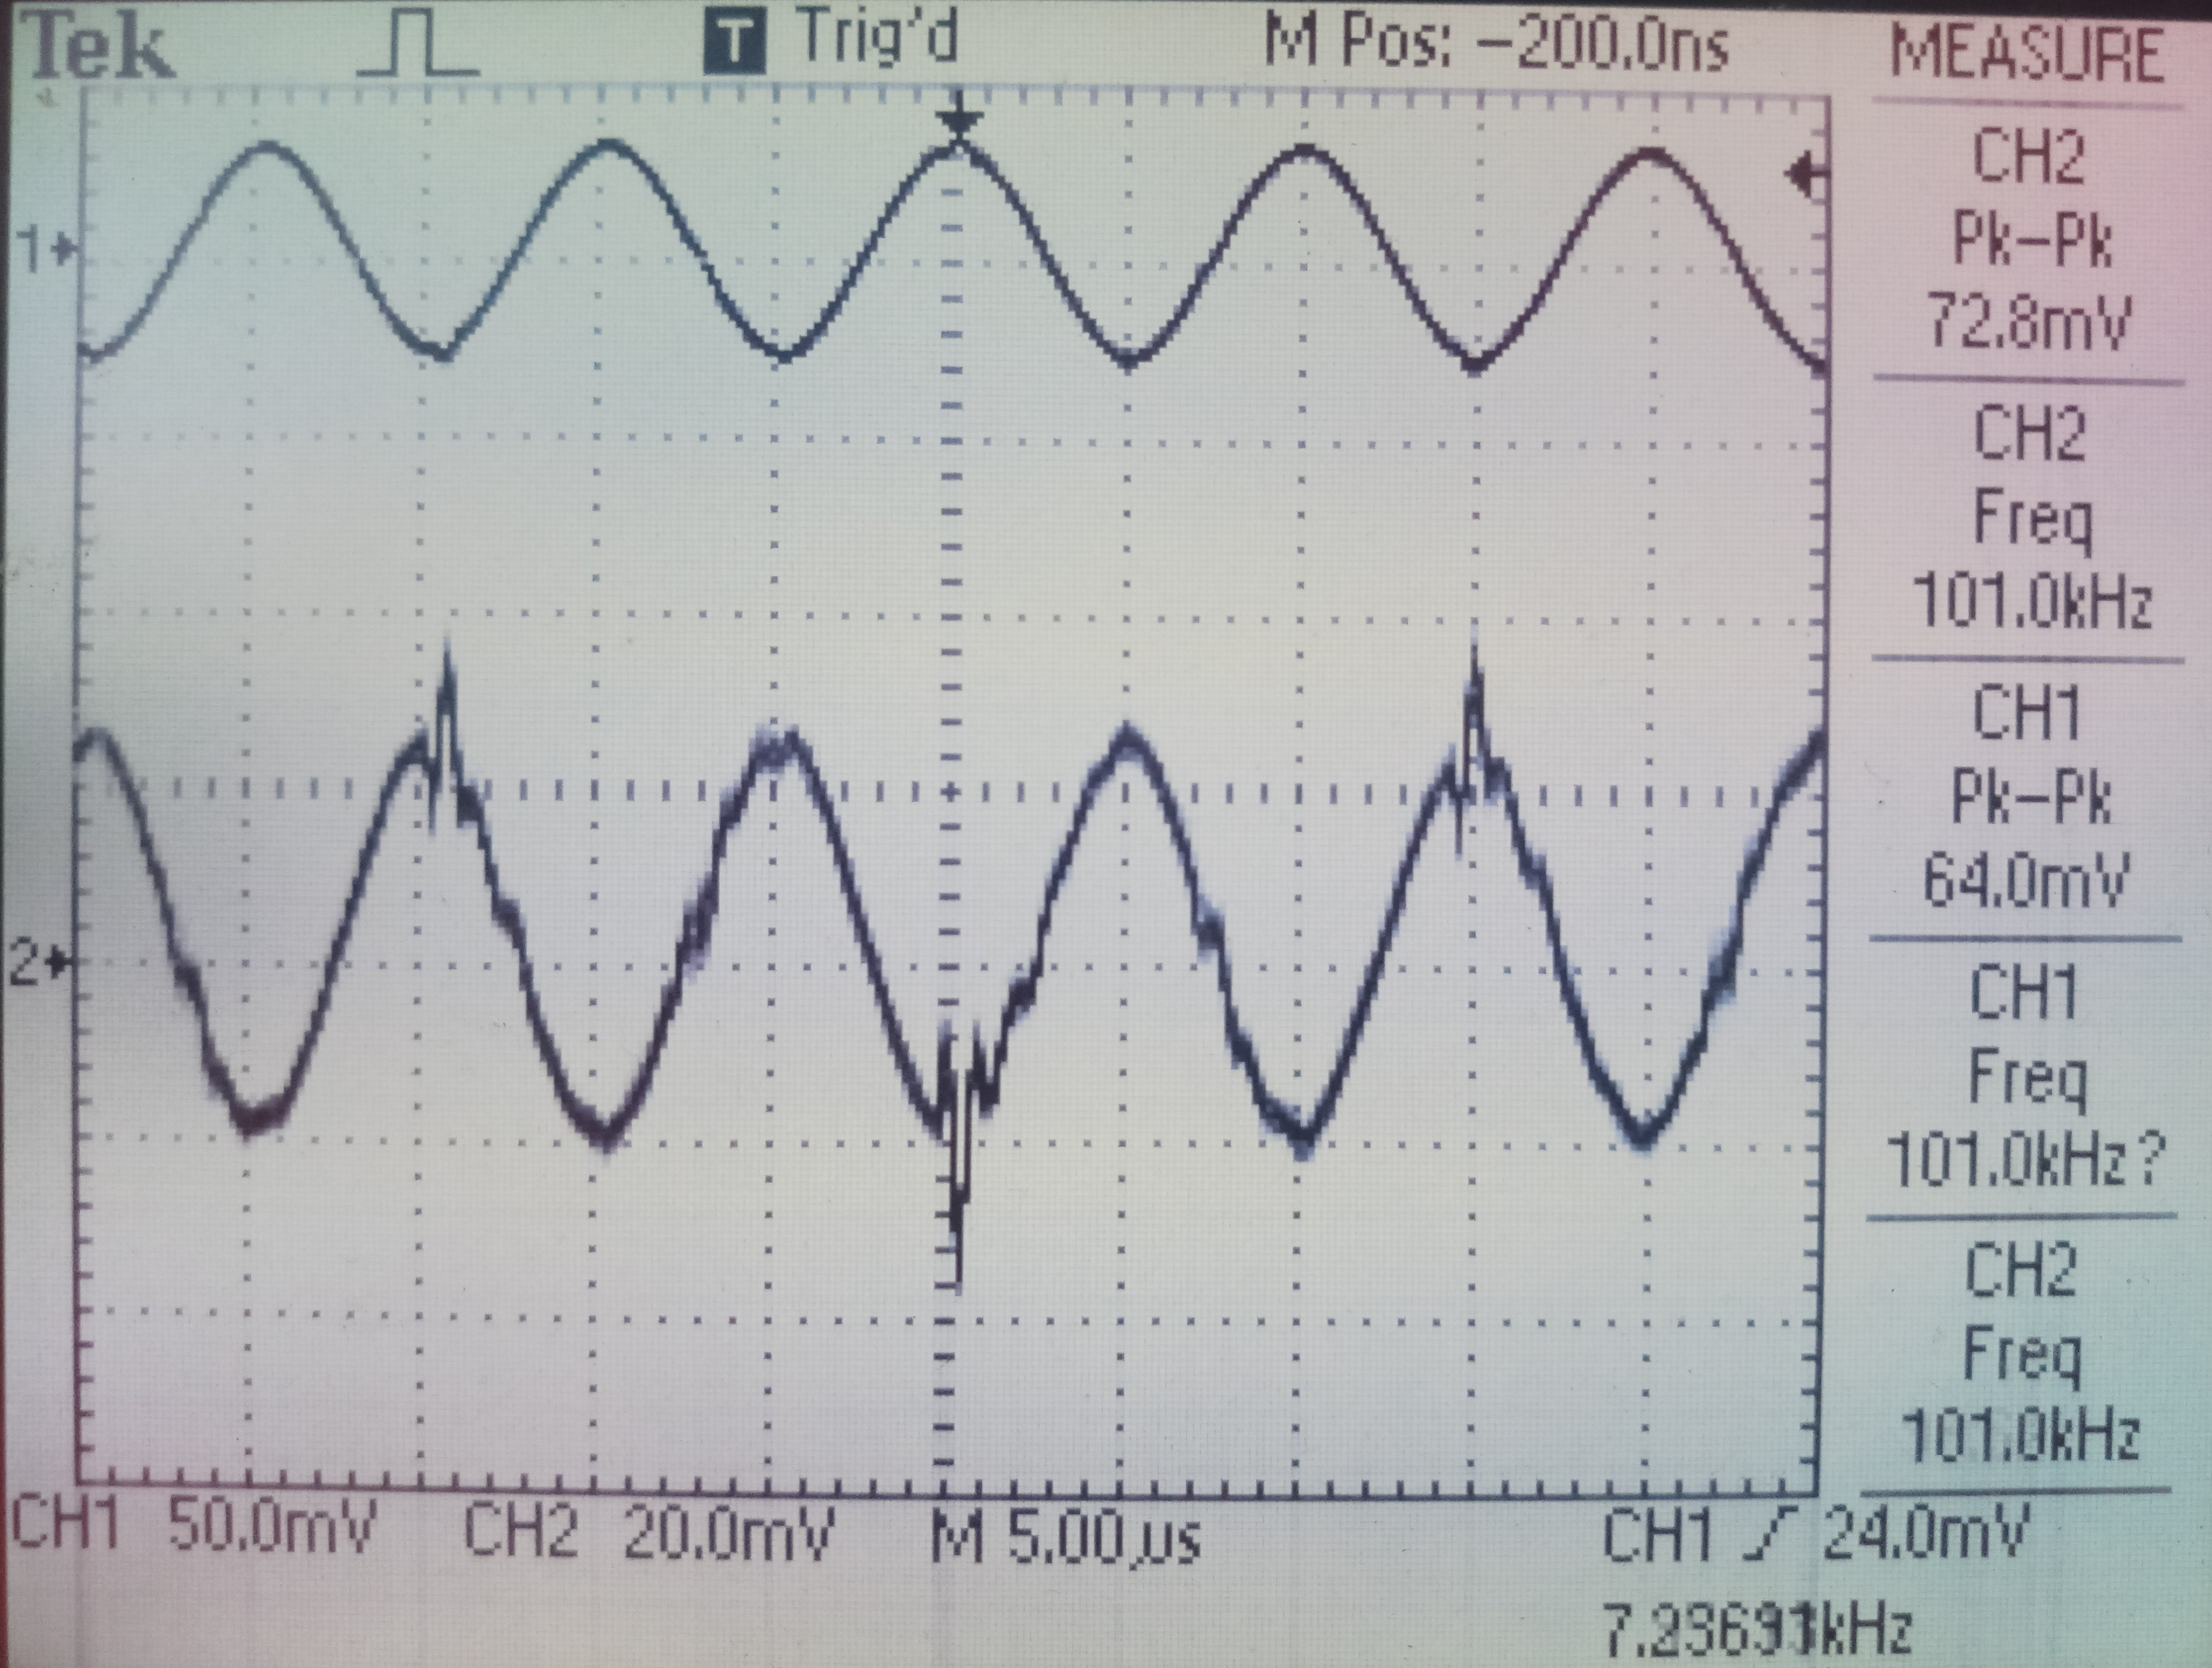
\includegraphics[width = 0.85\linewidth, trim = {0 0 0 0}, clip]{15_23_06.jpg}
		\caption{Observation 2}
	\end{subfigure}
	\begin{subfigure}[b]{\linewidth}
	   	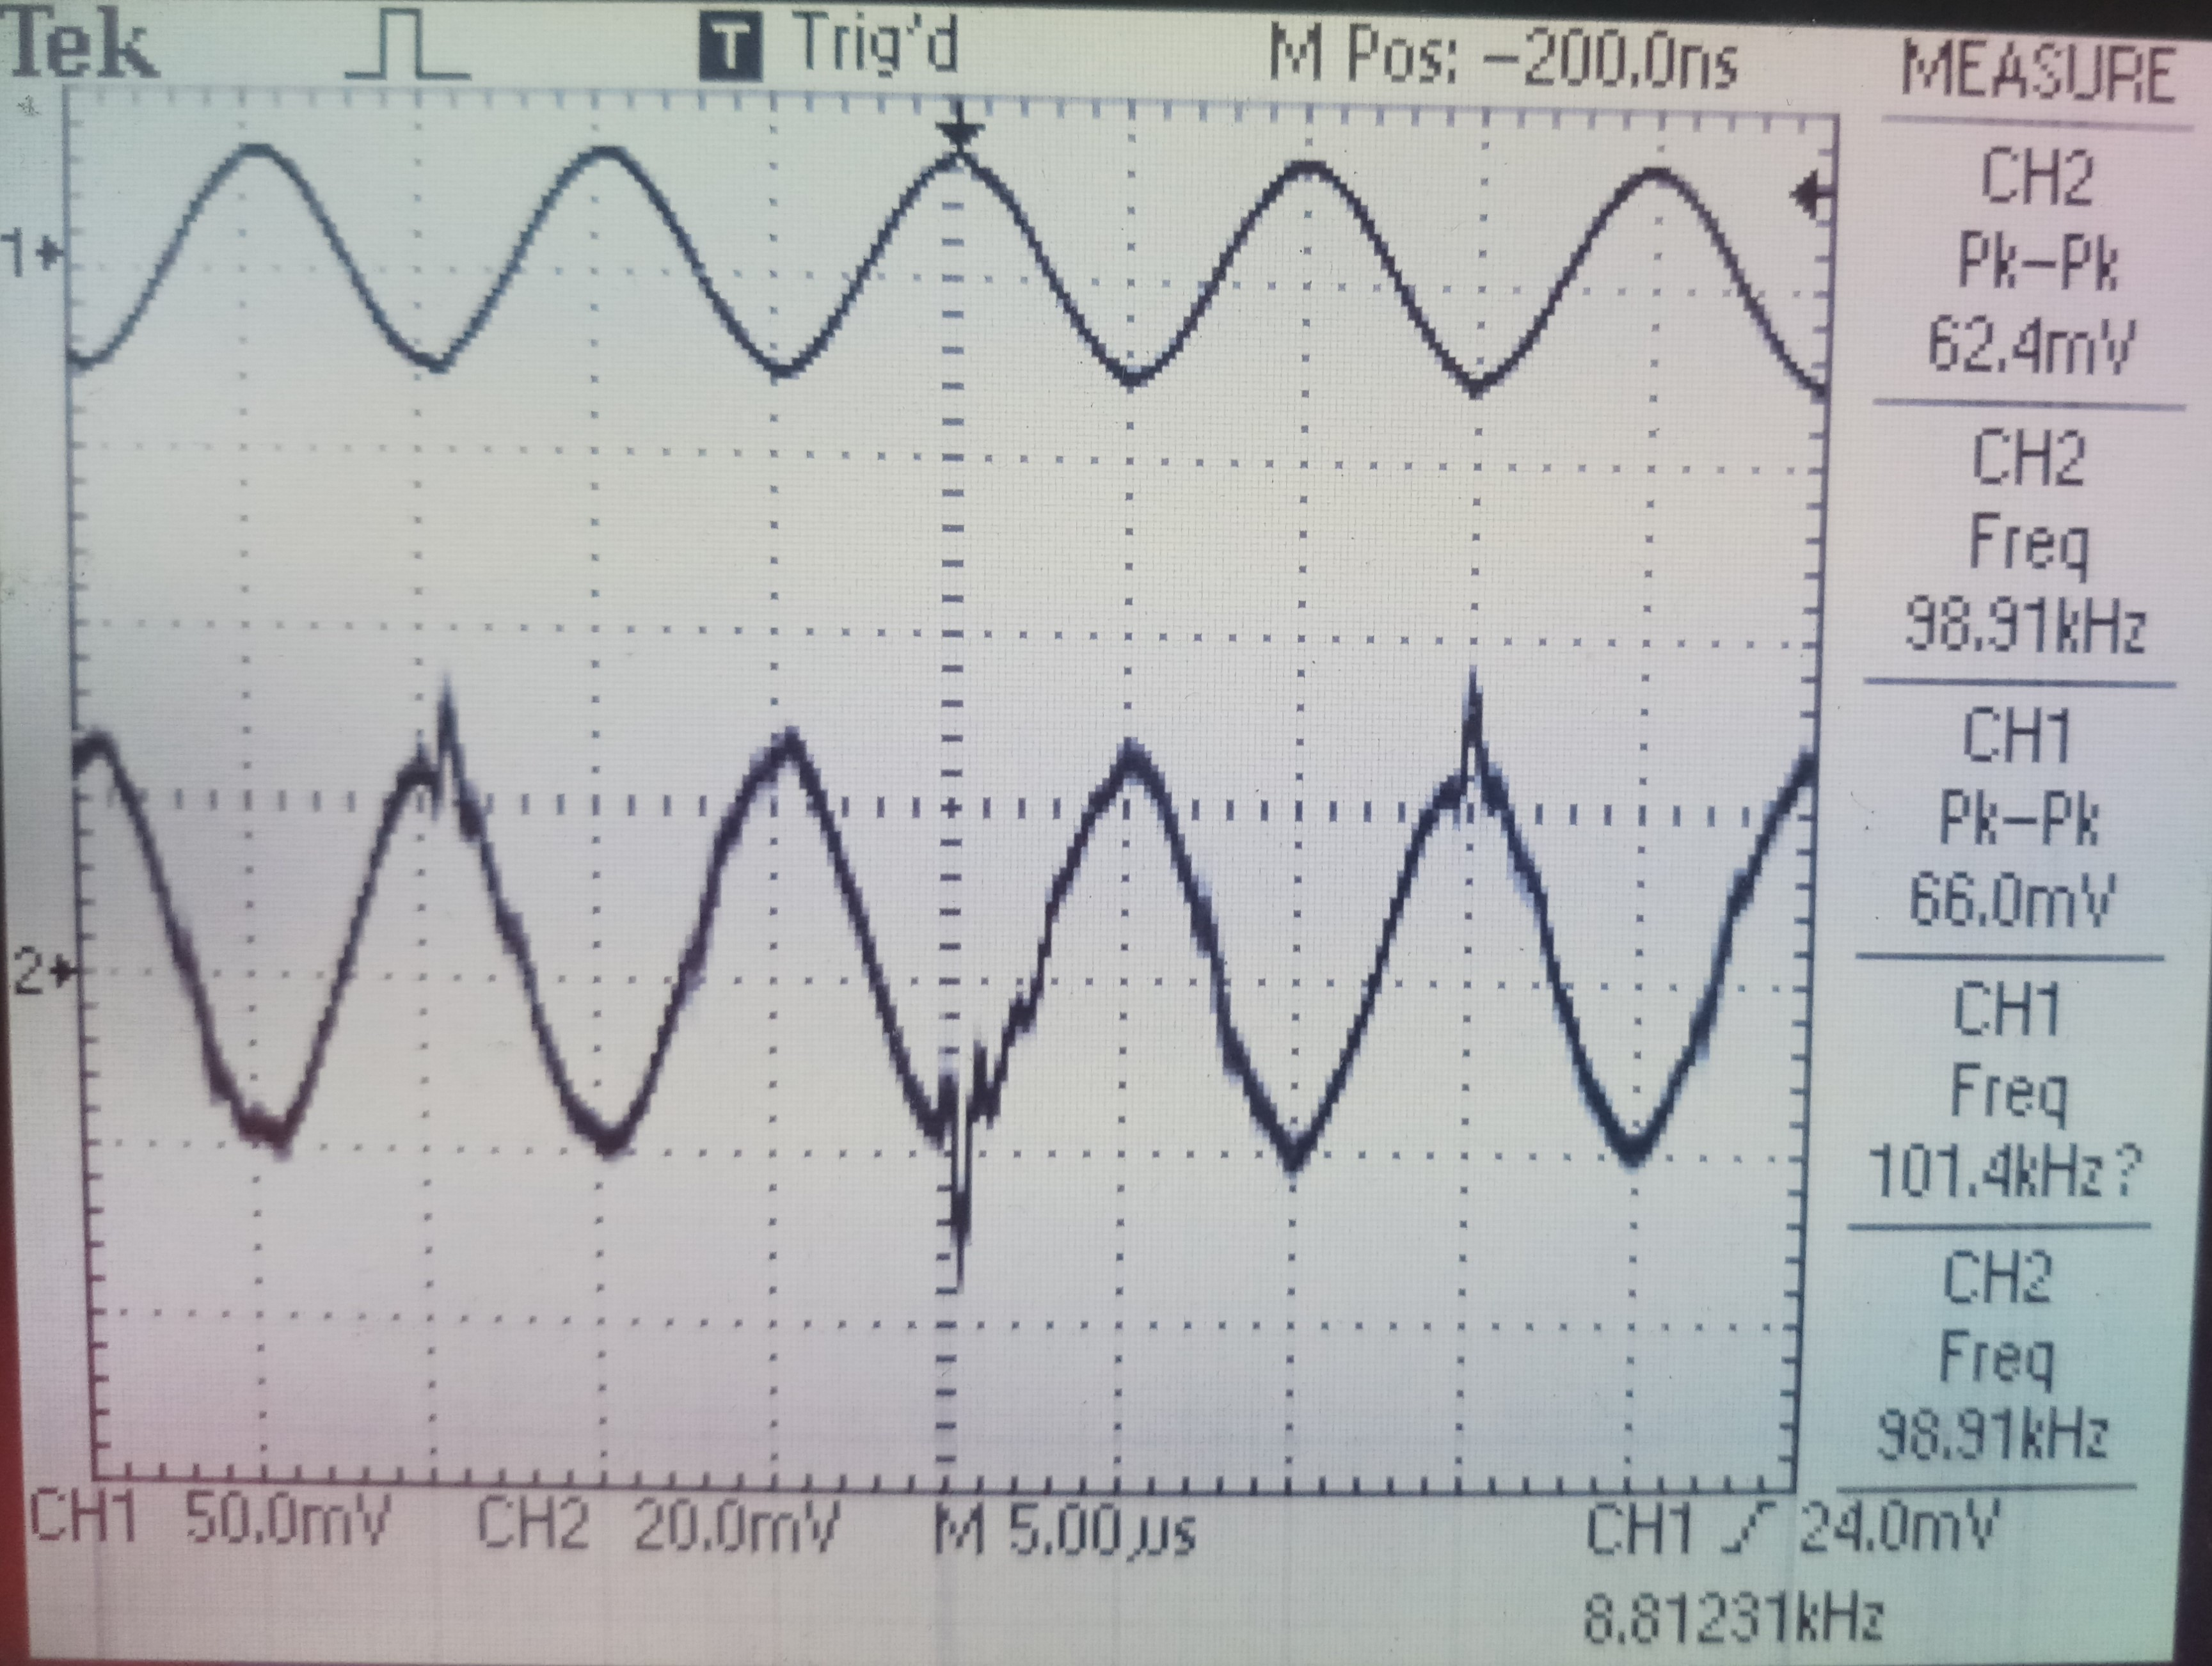
\includegraphics[width = 0.85\linewidth, trim = {0 0 0 0}, clip]{15_24_11.jpg}
		\caption{Observation 3}
	\end{subfigure}\\
	\caption{DUT Outputs (contd.)}
\end{figure}
\end{center}

Other observation images have not been added due to the limitation of 10MB while submitting the report.

\section{Code}
\begin{verbatim}
#include<iostream>
#include<math.h>
#include<algorithm>

using namespace std;

long double esi = 1.0447*pow(10,-10);
long double wt = 385.98*pow(10, -9);
long double q = 1.602176565*pow(10,-19);
long double ni = 9.817*pow(10,9);
long double k = 1.3806*pow(10, -23);
float T = 300.0;
long double c = (esi*k*T)/(q*q);
long double f1(long double x)
{
    return ((c*log(x/ni))/x)-(wt*wt/4);
}
long double fprime(long double x)
{
    return ((f1(x+0.01)-f1(x))/0.01);
}
int main()
{
    long double m = pow(10,14);
    while(f1(m)>(2*pow(10,-8))||f1(m)<(-2*pow(10,-8)))
        m = m-(f1(m)/fprime(m));
    cout<<m<<endl;
    return 0;
}
\end{verbatim}

\section{Simulation}
\begin{enumerate}
\item \textbf{Part 1}

\begin{verbatim}
I-D vs V_DS

.include ALD1107.txt

m1 1 2 0 0 ALD1107
vgg 3 0 dc -5V
r2 4 0 3k
r1 3 4 2k
r3 3 5 100
r4 5 0 1k
vdummy1 1 5 dc 0V
vdummy2 2 4 dc 0V 

.dc r4 1 10k 0.1
.control
run

plot i(vdummy1) vs v(1)

.endc
.end
\end{verbatim}


\item \textbf{Part 2}

\begin{verbatim}
I-D vs V_DS

.include ALD1107.txt

m1 1 2 0 6 ALD1107
vgg 3 0 dc -5V
r2 4 0 1.5k
r1 3 4 3.5k
r3 3 5 4.7k
r4 5 0 200
vdummy1 1 5 dc 0V
vdummy2 2 4 dc 0V 
vbs 6 0 dc 4V

.dc r2 1 5k 0.1
.control
run

plot i(vdummy1) vs v(2)

.endc
.end
\end{verbatim}

\item \textbf{ALD1107}

\begin{verbatim}
**ALD1107 SPICE Parameter File
.MODEL ALD1107 PMOS (LEVEL=1 CBD=0.5p CBS=0.5p CGDO=0.1p CGSO=0.1p GAMMA=.45
+ KP=100u L=10E-6 LAMBDA=0.0304 PHI=.8 VTO=-0.82 W=20E-6)
\end{verbatim}
\end{enumerate}

For part 1, based on the simulation and the data hence obtained, the following graph is shown below:

\begin{figure}[H]
	\centering
	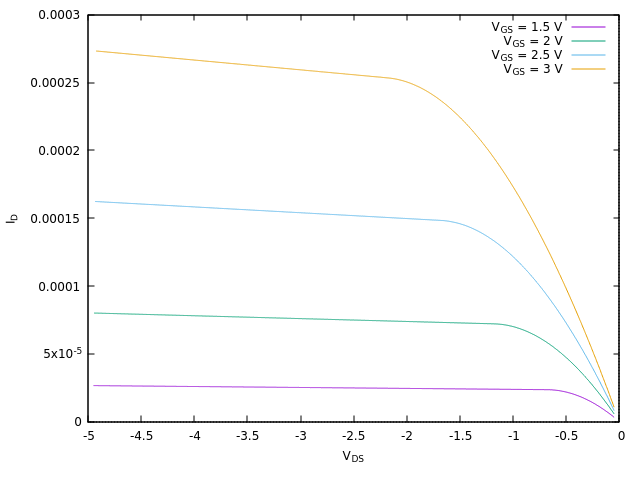
\includegraphics[width = \linewidth, trim = {0 0 0 0}, clip]{Part1.png}
	\caption{\(I_D\) vs \(V_{DS}\)}
\end{figure}

For part 2, based on the simulation and the data hence obtained, the following graph is shown below:

\begin{figure}[H]
	\centering
	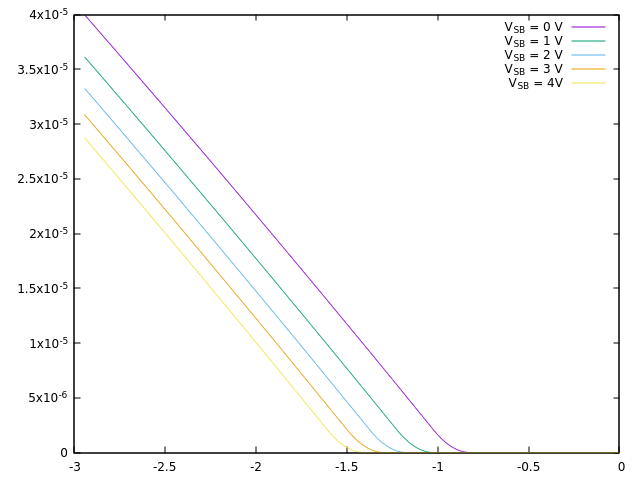
\includegraphics[width = \linewidth, trim = {0 0 0 0}, clip]{Part2.png}
	\caption{\(I_D\) vs \(V_{GS}\)}
\end{figure}

\section{Inference}
The oxide capacitance is given by the capacitance of the MOSCAP in the accumulation region which is equal to the maximum capacitance for high frequency measurements. Hence we have:
\[ C_{OX} =  \frac{355.99\ pF}{3.14159 \times (0.1\ cm)^2 / 4} = 45.326\ nF/cm^2 \]
From the oxide capacitance, we get oxide thickness \(d_{OX}\) since we have:
\[C_{OX} = \frac{\epsilon_{OX}}{d_{OX}}\]
which gives us:
\[d_{OX} = \frac{\epsilon_{OX}}{C_{OX}}\]
\[d_{OX} = \frac{0.34\ pF/cm}{45.326\ nF/cm^2} = 75.012\ nm\]

The minimum value of capacitance occurs in the inversion region. This capacitance is given by:
\[\frac{1}{C_{MIN}} = \frac{1}{C_{OX}} + \frac{1}{C_{S}} = \frac{230.77\ pF}{3.14159 \times (0.1\ cm)^2 / 4} = 29.383\ nF/cm^2\]
This gives us the value for \(C_{S}\):
\[C_{S} = \frac{1}{\frac{1}{C_{MIN}} - \frac{1}{C_{OX}}} = 83.533\ nF/cm^2\]
Also we can relate this capacitance to the required depletion region width \(W_T\):
\[C_{S} = \frac{\epsilon_{Si}}{W_T}\]
which gives us:
\[W_T = \frac{\epsilon_{Si}}{C_S}\]
\[W_T = \frac{1.0447\ pF/cm}{83.533\ nF/cm^2} = 125.064\ nm\]

From the value of \(W_T\), we may use the intrinsic formula relating the same to the doping concentration \(N_A\):
\[(W_T)^2 = \frac{\epsilon_S \times kT \times ln\left(\frac{N_A}{n_i}\right)}{q^2 \times N_A}\]
Here we use the code given below in order to find the value of \(N_A\):
\[N_A = 1.28217\times 10^{16}\ cm^{-3}\]
In order to find the Debye length, we use the following:
\[L_D = \left(\frac{\epsilon_{Si}kT}{q^2N_A}\right)^{0.5} = \left(\frac{(1.0447\ pF/cm) \times (4.1442\times10^{-9}\ pN.m)}{(1.602\times10^{-19}\ C)^2\times (1.28217\times 10^{16}\ cm^{-3})}\right)^{0.5} = 36.273 nm\]
This gives us \(C_{Debye}\):
\[C_{Debye} = \frac{\epsilon_{Si}}{L_D} = \frac{1.0447 pF/cm}{36.273 nm} = 288.0103\ nF/cm^{2}\]
And from \(C_{Debye}\), we may obtain the flat-band capacitance per unit area \(C_{FB}\) as follows:
\[C_{FB} = \frac{1}{\frac{1}{C_{OX}} + \frac{1}{C_{Debye}}} = \frac{1}{\frac{1}{45.326\ nF/cm^2} + \frac{1}{288.0103\ nF/cm^2}} = 39.163\ nF/cm^2\]
Hence we get the flat-band voltage \(V_{FB}\) as the voltage matching C = 311.647 pF:
\[V_{FB} \approx -2.10 V\]
Here, C is the flat-band capacitance (\(C_{C_{FB}}\)):
\[C_{C_{FB}} = 311.647\ pF\]\\

Hence we have obtained the required parameters:\\
Oxide Capacitance, \(C_{OX} = 45.326\ nF/cm^2 \)\\
Oxide thickness, \(d_{OX} = 75.012\ nm\)\\
Flat-band capacitance, \(C_{FB} = 39.163\ nF/cm^2\)\\
Flat-band voltage, \(V_{FB} = -2.10 V\)

\end{document}
